\documentclass{article}

\usepackage[english]{babel}
\usepackage[utf8]{inputenc}
\usepackage{amsmath,amssymb}
\usepackage{tabularx}
\usepackage{booktabs}
\usepackage{enumitem}
\usepackage{parskip}
\usepackage{graphicx}
\usepackage{fancyvrb}
\usepackage{alltt}
\usepackage{float}
\usepackage[top=2.5cm, left=3cm, right=3cm, bottom=4.0cm]{geometry}

\newcommand{\lectureheader}[4]{%
  \begin{minipage}{.3\textwidth}%
    
    \strut
\includegraphics[width=\textwidth]{figures/ethlogo.pdf}%
  \end{minipage} \hfill%
  \raisebox{1.5mm}{%
    \begin{minipage}{0.69\textwidth}\sf\flushright%
        \textbf{\Huge #3}\mbox{\hspace{2mm}}\\#4\mbox{\hspace{2mm}}%
    \end{minipage}%
  }\\[-2mm]\hrule%
  \begin{minipage}[t]{0.5\textwidth}\sf\textit{#1} \end{minipage} \hfill%
  \begin{minipage}[t]{0.5\textwidth}\sf\flushright \textit{#2}\end{minipage}%
  \par%
}

% Create commands for syntax that you will frequently use
\newcommand{\xx}{\mathbf x}

\begin{document}
\begin{titlepage} 

\lectureheader{Prof. Ryan Cotterell}
{}
{\Large Natural Language Processing}{Spring 2021}
	\newcommand{\HRule}{\rule{\linewidth}{0.5mm}} 
	
	\center % Centre everything on the page
	{\Huge Course Assignment}\\
      \quad\newline
	
	{\large\today} \\
	\quad\newline
	%	Author
	%------------------------------------------------
	
	{\Large Karol Borkowski \\ \emph{nethz} Username: kborkowski \\ Student ID: 20-905-501}\\[0.5cm] 
	\vfill
	{\large \textbf{Collaborators:} \\
	Sven Kohler}
	
	\vfill\vfill\vfill 
	By submitting this work, I verify that it is my own. That is, I have written my own solutions to each problem for which I am submitting an answer. I have listed above all others with whom I have discussed these answers.
	
	\vfill 
	
\end{titlepage}


\part{Course Assignment Episode 1}

\section*{Question 1} 
\begin{enumerate}[label = (\alph*)]
    \item
    
\begin{figure}[h!]
    \centering
    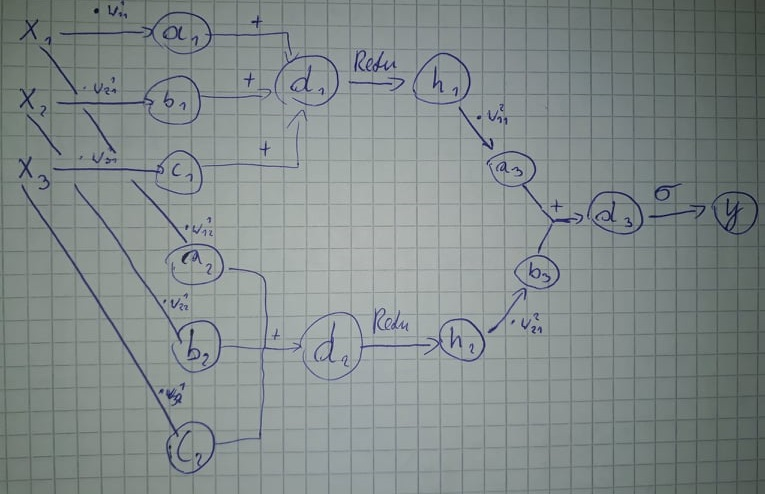
\includegraphics[scale=1.5]{figures/backprop.jpg}
    \caption{The computation graph of f.}
\end{figure}

$a_1 = x_1 \cdot w_{11}^1 \; \;$
$b_1 = x_2 \cdot w_{21}^1 \; \;$
$c_1 = x_3 \cdot w_{31}^1 \; \;$

$d_1=a_1 + b_1 + c_1$

$h_1 = ReLu(d_1)$

$a_2 = x_1 \cdot w_{12}^1 \; \;$
$b_2 = x_2 \cdot w_{22}^1 \; \;$
$c_2 = x_3 \cdot w_{32}^1 \; \;$

$d_2=a_2 + b_2 + c_2$

$h_2 = ReLu(d_2)$

$a_3 = h_1 \cdot w_{11}^2 \; \;$
$b_3 = h_2 \cdot w_{21}^2 \; \;$

$d_3=a_3 + b_3$

$y=\sigma(d_3)$

\item 
	\begin{enumerate}[label = (\roman*)]
		\item
		$h_1=ReLu(1+1+1) = 3 \; \;$
		$h_2=ReLu(1+1+1) = 3 $
		
		$y=\sigma(3+3) \simeq 0.99753$
		
		\item
		$\frac{\partial L}{\partial \hat{y}} = \frac{-y}{\hat{y}}-\frac{1-y}{1-\hat{y}}\simeq -404 \; \; \;$ 
		
		$\frac{\partial y}{\partial d_3} = \sigma(d_3) \cdot (1-\sigma(d_3)) \simeq 0.00247 \; \; \;$
		
$\frac{\partial d_3}{\partial a_3} = 1 $ 

$\frac{\partial d_3}{\partial b_3} = 1 \; \; \;$ 

$\frac{\partial a_3}{\partial w_{11}^2} = h_1 = 3 \; \; \;$ 

$\frac{\partial b_3}{\partial w_{21}^2} = h_2 = 3 \; \; \;$

$\frac{\partial a_3}{\partial h_1} = w_{11}^2 = 1 $

$\frac{\partial b_3}{\partial h_2} = w_{21}^2 = 1 $

$\frac{\partial h_1}{\partial d_1} = 1 $

$\frac{\partial h_2}{\partial d_2} = 1 $

$\frac{\partial d_1}{\partial a_1} = 1 $

$\frac{\partial d_1}{\partial b_1} = 1 $

$\frac{\partial d_1}{\partial c_1} = 1 $

$\frac{\partial d_2}{\partial a_2} = 1 $

$\frac{\partial d_2}{\partial b_2} = 1 $

$\frac{\partial d_2}{\partial c_2} = 1 $

$\frac{\partial a_1}{\partial w_{11}^1} = 1 $

$\frac{\partial b_1}{\partial w_{21}^1} = 1 $

$\frac{\partial c_1}{\partial w_{31}^1} = 1 $

$\frac{\partial a_2}{\partial w_{12}^1} = 1 $

$\frac{\partial b_2}{\partial w_{22}^1} = 1 $

$\frac{\partial c_2}{\partial w_{32}^1} = 1 $

$\frac{\partial a_1}{\partial x_1} = 1 $

$\frac{\partial b_1}{\partial x_2} = 1 $

$\frac{\partial c_1}{\partial x_3} = 1 $

$\frac{\partial a_2}{\partial x_1} = 1 $

$\frac{\partial b_2}{\partial x_2} = 1 $

$\frac{\partial c_2}{\partial x_3} = 1 $
		
		
		
		\item
		$\frac{\partial L}{\partial \hat{y}} = \frac{-y}{\hat{y}}-\frac{1-y}{1-\hat{y}}\simeq -404 \; \; \;$ 
		
		\item
		$\Delta w_{ij} = -\eta \frac{\partial L}{\partial w_{ij}}$
		
		$\frac{\partial L}{\partial w_{11}^2} = \frac{\partial L}{\partial \hat{y}} \cdot \frac{\partial \hat{y}}{\partial d_3}  \cdot \frac{\partial d_3}{\partial w_{11}^2} = -0.99788$
		
$\Delta w_{11}^2 = 0.1 \cdot -0.99788 = -0.099788$
		
		$\frac{\partial L}{\partial w_{21}^2} = \frac{\partial L}{\partial \hat{y}} \cdot \frac{\partial \hat{y}}{\partial d_3}  \cdot \frac{\partial d_3}{\partial w_{21}^2} = -0.99788$
		
$\Delta w_{21}^2 = 0.1 \cdot -0.99788 = -0.099788$

		$\frac{\partial L}{\partial w_{11}^1} = \frac{\partial L}{\partial \hat{y}} \cdot \frac{\partial \hat{y}}{\partial d_3}  \cdot \frac{\partial d_3}{\partial a_3} \cdot \frac{\partial a_3}{\partial h_1 } \cdot \frac{\partial h_1}{\partial d_1} \cdot \frac{\partial d_1}{\partial a_1} \cdot \frac{\partial a_1}{\partial w_{11}^1} = -0.99788$
		
$\Delta w_{11}^1 = 0.1 \cdot -0.99788 = -0.099788$

Since the input values are the same and the weight values are also the same, the rest of the gradient changes have the same value. The calculation are analogous to the above ones. 
	
				
	\end{enumerate}
	
	\item
	The symmetry of weights is not broken, so the hidden units can be replaced with a single unit producing the same output. The benefits of such solution are: faster training, more reliable model due to fewer parameters.

\end{enumerate}



\clearpage
\newpage
\section*{Question 4} 
\begin{enumerate}[label = (\alph*)]
    \item
    \begin{enumerate}[label = (\roman*)]
    \item
    Let's define an auxiliary function $J_w = \begin{cases}
      1, & \text{if} \; w \; is \; drawn \\
      0, & \text{otherwise}
    \end{cases}$
    
    The number of unique tokens X is equal to:
    
    $X = \sum_{w=1}^{|V|} J_w$
    
    Using the linearity of expectations, the expected value of X is equal to:
    
    $E[X] = E[\sum_{w=1}^{|V|} J_w] = \sum_{w=1}^{|V|} E[J_w]$
    
    where:
    
    $E[j_w] = P(J_w = 1) = P(at \;least\; one\; w \;selected) = 1 - P(w \; not \; selected) = 1- \frac{|V|-1}{|V|}$
    
    Finally: $X = |V| \cdot (1 - \frac{|V|-1}{|V|})^n$
    
    \item
    P(all words appear) = 1 - P(at least one w doesn't appear) = $1 - (P(!w_1) \bigcup P(!w_2) \bigcup ... \bigcup P(!w_|V|) = 1 - |\bigcup_{i=1}^{|V|}P(!w_i)|)$ 
    
    where '!' denotes that the word is not selected. 
    The above union can be found using the inclusion-exclusion principle. 
    
    $|\bigcup_{i=1}^{|V|}P(!w_i)| = \sum_{J \in \{1,...,|V|\}} (-1)^{|J|+1}|\bigcup_{j \in J}P(!w_i)|) $
    
	\end{enumerate}
	
	\item
    \begin{enumerate}[label = (\roman*)]
    \item
    A - expected additional draws if just selected any word other than 'work'
    
    B - expected additional draws if just selected 'work'

	A is equal to the initial draw + P(w != 'hard') * A + P(w = 'hard') * B, what yields:
	
	$A = 1 + \frac{|V|-1}{|V|} \cdot A + \frac{1}{|V|} \cdot B$   
	
	B is equal to one draw in case that we select word 'hard' + P(w != 'hard') * A, what yields: 
	
	$B = 1 + \frac{|V|-1}{|V|} \cdot A$
	
	Solving the above system of equations in terms of A, we get:
	
	$A = \frac{|V|^2-1}{|V|-1}$ 
    
    \item
    Probability that the word "work" is selected in n draws is equal to 1 - probability that it is not selected. 
    
    $P('work' 
   \; selectes) = 1 - P('work' \; not \; selected) = 1 - (\frac{|V|-1}{|V|})^n$
   
   To find the expected number of draws let's put 0.95 for P and solve the above equation for variable n:
   
   $1 - (\frac{|V|-1}{|V|})^n \geq 0.95$
   
   $(\frac{|V|-1}{|V|})^n \leq 0.05$
   
   $n \leq log_{\frac{|V|-1}{|V|}}(0.05)$
    
	\end{enumerate}
	
	\item
    \begin{enumerate}[label = (\roman*)]
    \item
    A - expected number of draws before the first selection
    
    B - expected additional number of draws after at least one word has been selected.
    
    A is equal to B + the initial draw:
    
    $A=B+1$
    
    B is equal to P(w is the same as the previous one) + P(w is different) * A:
    
    $B = \frac{1}{|V|} + \frac{|V|-1}{|V|} \cdot A$
    
    The solution of the above set of equations in terms of A is:
    
    $A = |V|+1$
    
    \item
    I assume that the input is an integer corresponding to a given word index.
    
    $w_0=1$
    
    $w_1=-1$
    
    $w_2=0$
    
    $w_0=0$
    
    $b_0=0$
    
    $f(x)=\begin{cases}
      1, & \text{if} \; x=0\\
      0, & \text{otherwise}
    \end{cases}$
    
    $g(x) = x$
    
    \item
    $w_3=1$
    
    $w_4=1$
    
    $w_5=1$
    
    $b_2=0$
    
    $b_0=0$
    
    $g(x) = x$
    
    $h(x) = x$
    
    A non-linear activation is required because the output cannot be express as a linear function of the inputs. It is similar to the XOR problem. 
    
    \item
    A non-uniform has a yields greater chances of sequentially drawing the same token. 
    In can be intuitively depicted using an extreme case, when always the same word is drawn. 
    
	\end{enumerate}
    
\end{enumerate}


\clearpage
\newpage
\section*{Question 5} 
\begin{enumerate}[label = (\alph*)]
    \item
    \begin{enumerate}[label = (\roman*)]
    \item
    G = $<V, E, W>$
    
    E - associations between two consecutive words
    
    W = $score_{w} - score_{max}, \; for \; each \; w \; \in \; vocabulary $  
    
    To solve the decoding problem we need to find the highest scoring path, what is equivalent to finding the longest path on a graph with negative weights. The negativity of the weights is ensured using the above transformation for W. 
    The following algorithm is guaranteed to work only in the case of a directed trelis.
    
    \begin{Verbatim}[tabsize=4]
    	def Dijkstra(G, W, src):
    		# preparation
    		Q = prior_queue()
    		dist = map(cardiality(G))
    		back_ptrs = map(cardiality(G))
    		for v in G:
    			if v == src: 
    				disv[v] = 0
    			else:
    				dist[v] = inf
    			back_ptrs[v] = null
    			Q.add(src, dist(src))
    			
    		#main part
    		while !Q.is_empty():
    			u = Q.get_min()
    			for v in neighbours(u):
    				d = dist[u] + W[V]
    				if d < dist[v]:
    					dist[v] = d
    					back_ptrs[v] = u
    					Q.decrease_prior(v, d)
    		return dist, back_ptrs
    	\end{Verbatim}
    	
    	\item
    	Dijkstra: $O((|V|+|E|) \cdot log(|V|))$
    	
    	Viterbi: $O(T^2 \cdot |S|) = O(|E|)$
    	
    	Dijkstra algorithm is faster under the following condition:
   
    	 $(|V|+|E|) \cdot log(|V|) < |E|$
    	
	\end{enumerate}
	
	\item
	
	\begin{enumerate}[label = (\roman*)]
    \item
       \begin{alltt}
    	def Dijkstra(G, W, src):
    	    # preparation
    	    ...
    	    #main part
    	    while !Q.is_empty():
    	        u = Q.get_min()
    	        for v in neighbours(u):
    	            d = \(\bigoplus \)(dist[u] \(\bigotimes \) W[v])
    	            dist[v] = d
    	            back_ptrs[v] = arg(d)
                Q.decrease_prior(v, d)
         return dist, back_ptrs
    	\end{alltt}
    	
    Used semiring: 
    
    In case of positive weights and the shortest path: $<R^+ \bigcup \{\inf\}, min, +, \inf, 0>$
    
    The case of the longest path and negative weights is shown in thpoint ii).     
    
    \item
    $<R^- \bigcup \{- \inf\}, max, +, -\inf, 0>$
    
    \item
    $<R^+ \bigcup \{\inf\}, max, min, 0, \inf>$
    
    \end{enumerate}
 	    
\end{enumerate}

\clearpage
\newpage
\part{Course Assignment Episode 2}

\section*{Question 1} 
\begin{enumerate}[label = (\alph*)]
    \item
    $<N, \Sigma, R, S>$
    
    N = {NP, VP, PP, V, NP, Det, N, P}
    
    $\Sigma$ = {I, draw, a, man, with, pencil, hit, ball, an, umbrella, glasses}
    
    R:  
    
    $S \to NP \;\; VP$
    
    $NP \to Det \;\; N$
    
    $NP \to Np \;\; PP$
    
    $V \to VP \;\; PP$
    
    $VP \to V \;\; NP$
    
    $PP \to P \;\; NP$
    
    $NP \to J \; | \; glasses$
    
    $V \to draw \; | \; hit$
    
    $Det \to a \; | \; an$
    
    $N \to man \; | \; pencil \; | \; ball \; | \; umbrella$
    
    $P \to with$
    
    \item
    $S \to NP \;\; VP$: 1
    
    $NP \to Det \;\; N$: 1/2
    
    $NP \to Np \;\; PP$: 1/7
    
    $NP \to J$: 2/7
    
    $NP \to glasses$: 1/14
    
    $V \to draw$: 1/2
    
    $V \to hit$: 1/2
    
    $Det \to a$: 6/7
    
    $Det \to an$: 1/7
    
    $N \to man$: 4/7
    
    $N \to pencil$: 1/7
    
    $N \to ball$: 1/7
    
    $N \to umbrella$: 1/7
    
    $P \to with$: 1
    
    $PP \to P \;\; NP$: 1
    
    $VP \to VP \;\; PP$: 1/3
    
    $VP \to V \;\; NP$: 2/3
    
    
    
    \item
    To capture different expansions of NP, we introduce the the following rules:
    
    $NP \to N$ and $N \to J$
    
    The new PCFG is:
    
    $S \to NP \;\; VP$: 1
    
    $NP \to Det \;\; N$: 1/2
    
    $NP \to Np \;\; PP$: 1/7
    
    $NP \to N$: 5/14
    
    $V \to draw$: 1/2
    
    $V \to hit$: 1/2
    
    $Det \to a$: 6/7
    
    $Det \to an$: 1/7
    
    $N \to man$: 4/12
    
    $N \to pencil$: 1/12
    
    $N \to ball$: 1/12
    
    $N \to umbrella$: 1/12
    
    $N \to J$: 5/12 
    
    $P \to with$: 1
    
    $PP \to P \;\; NP$: 1
    
    $VP \to VP \;\; PP$: 1/3
    
    $VP \to V \;\; NP$: 2/3
     
	\begin{figure}[H]
	\item
    \centering
    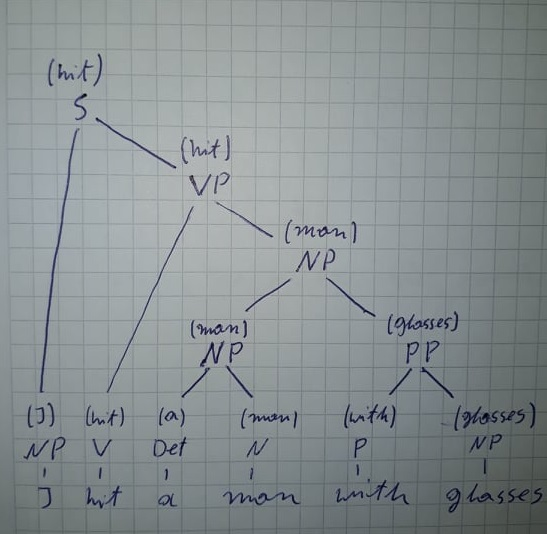
\includegraphics[scale=1.5]{figures/tree.jpg}
    \caption{The parse tree for the sentence “I hit a man with glasses” with 		lexicalized rules.}
	\end{figure}
	
	\item
	The time complexity of CKY algorithm is $O(n^3 \cdot |G|)$, 
	where n is the length of the parsed string and $|G|$ is the size of the CNF grammar G.
	
	The modifications from parts c) and d) increases the number of the grammar rules $|G|$ and therefore the time of the algorithm execution. Nevertheless, the order expressed by the big-O notation is the same. 
	
	The space complexity of the CKY algorithm is determined by the size of the used matrix, which is: $O(n^2)$
     
\end{enumerate}


\clearpage
\newpage
\section*{Question 2} 
\begin{enumerate}[label = (\alph*)]
    \item
    Let's create a lexicalized production for each $\psi(i \to j)$,
     
    where i $<$ j: 
    
    $X(w_i) \to X(w_i)X(w_j) \; : \; \psi(i \to j)$,
    
    where i $>$ j: 
    
    $X(w_i) \to X(w_j)X(w_i) \; : \; \psi(i \to j)$
    
    and for each $\psi(root \to j)$:
    
    $S \to X(w_j) \; : \; \psi(root \to j)$
    
    \item
    Let's consider all possible dependency parses and their associated
derivations in the lexicalized CFG:

	$\psi_\tau(y^1) = \psi_\tau(S \to X(They)) + \psi_\tau(X(They) \to X(They X(fish))) = \psi(root \to 1) + \psi(1 \to 2) = \Psi(1 \to 2)$
	
		$\psi_\tau(y^2) = \psi_\tau(S \to X(fish)) + \psi_\tau(X(fish) \to X(They X(fish))) = \psi(root \to 2) + \psi(2 \to 1) = \Psi(2 \to 1)$
    
\end{enumerate}

\clearpage
\newpage
\section*{Question 4} 

\begin{enumerate}[label = (\alph*)]
    
\begin{table}[h]
\item
        \centering
        \fontsize{10}{10}\selectfont
        \renewcommand{\arraystretch}{1.2} % vertical padding
        \setlength{\tabcolsep}{0.5em} % for the horizontal padding
        \begin{tabular}{l|l|l|l}
        \textbf{number} & \textbf{sample strings} & \textbf{accepted} & \textbf{weight} \\ \hline
        1 & educational is this not & NO &  \\
        2 & is this assignment educational & NO  &  \\
        3 & not educational is not educational & YES  & 12  \\
        4 & this assignment is not educational &  YES & 9  \\
        5 & is this assignment educational & NO &  \\
        6 & this assignment course is educational & NO  &  \\
        7 & is this assignment not educational & YES & 15  \\
        8 & this assignment not & YES & 8  \\
        9 & this course assignment is not educational & YES & 12  \\
        10 & this course is not not educational & YES & 21 \\
        11 & not educational is this & YES & 11 \\
        12 & course assignment is not educational & YES & 10 \\
        13 & not this assignment is educational & NO &  \\
        14 & not not not educational & YES & 25 \\
        14 & is this course assignment not educational & YES & 25 \\
        15 & course assignment is this & 15 & 8 \\
        16 & this course is interesting & NO &  \\
        17 & this course assignment not educational & YES & 14
        \end{tabular}
        \caption{Some strings from $\mathcal{Y}_{\geq 2, \leq 6}$}
        \label{tab:wfst_strings}
        \end{table}
      
\begin{figure}[H]
		\item
        \centering
        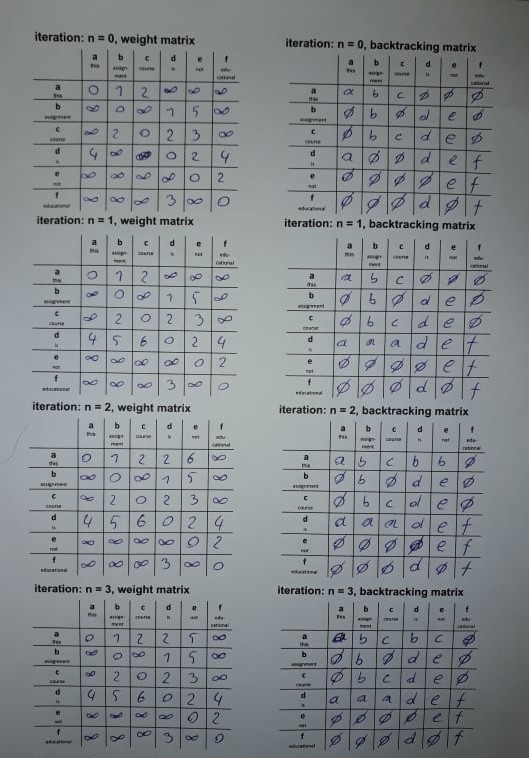
\includegraphics[width=1.0\textwidth]{./figures/floyd1.jpg}
        % \includegraphics[width=.45\linewidth]{./fig/C1000.png}
        \caption{Floyd-Warshall algorithm, iteration 0 to 3; left column matrix should contain weights after iteration n; right column matrix should be iteratively filled for backtracking each path}
        \label{fig:wfst_charts_1}
    \end{figure} 
    
    \begin{figure}[H]
        \centering
        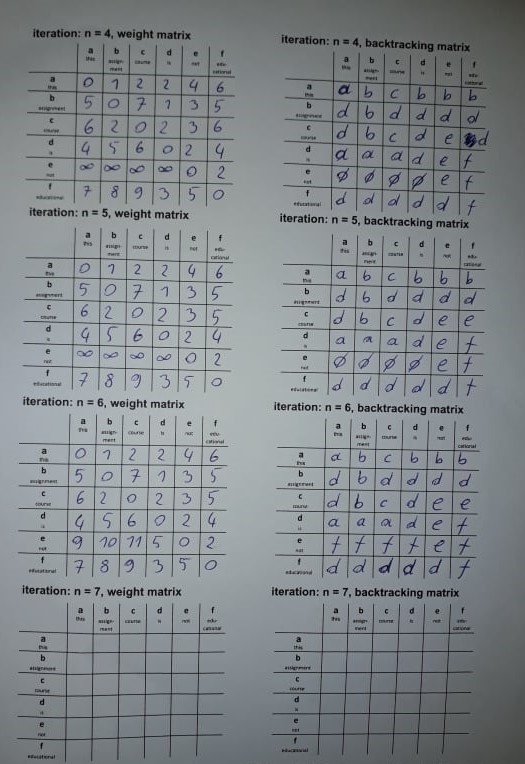
\includegraphics[width=1.0\textwidth]{./figures/floyd2.jpg}
        % \includegraphics[width=.45\linewidth]{./fig/C1000.png}
        \caption{Floyd-Warshall algorithm, iteration 4 to 7; left column matrix should contain weights after iteration n; right column matrix should be iteratively filled for backtracking each path}
        \label{fig:wfst_charts_2}
    \end{figure} 
    
	\item
	The number of iterations is bound by the number of nodes. It terminates after n=$|V|$
	
	\item    
	Time complexity: three for loops $=> \; O(n^3)$
	
	Space complexity: size of the matrices = $ 2 \cdot n^2 \; => \; O(n^2)$
	
	Backtracking: Maximal when all edges are included into the path $=> \; O(|E|)$
    
    \end{enumerate}
\end{document}
